\documentclass[reqno, 12pt]{amsart}

%%%%%%%%%% Packages %%%%%%%%%%

\usepackage{amsmath,bbm,verbatim,wasysym,nicefrac,amssymb,braket}
%mathtools,appendix,soul,ulem,slashed,upgreek
\usepackage[protrusion=true, babel=true]{microtype}
\usepackage[english]{babel}
\usepackage[widespace]{fourier}
\usepackage[backrefs]{amsrefs}
\usepackage[margin=1in]{geometry}
\usepackage[onehalfspacing]{setspace}
\usepackage[pdfusetitle,pagebackref]{hyperref}
\numberwithin{equation}{section}                % must be called before cleveref
\usepackage[nameinlink,noabbrev]{cleveref}
\expandafter\def\csname ver@etex.sty\endcsname{3000/12/31}
\let\globcount\newcount
\usepackage{autonum}                            % must be called after cleveref
\usepackage[dvipsnames]{xcolor}
\usepackage{tikz}
\usetikzlibrary{quantikz}
\usetikzlibrary{shapes.geometric, arrows}
\usepackage{subcaption}

\tikzstyle{process} = [rectangle, minimum width=3em, minimum height=2em, text centered, draw=blue, fill=gray!10]
\tikzstyle{startend} = [ellipse, minimum width=2em, minimum height=1em, text centered, draw=red, fill=gray!10]
\tikzstyle{arrow} = [thick,->,>=stealth]

%%%%%%%%%% align break fix %%%%%%%%%%

\allowdisplaybreaks[1]

%%%%%%%%%% Left/Right fix %%%%%%%%%%

\let\originalleft\left
\let\originalright\right
\renewcommand{\left}{\mathopen{}\mathclose\bgroup\originalleft}
\renewcommand{\right}{\aftergroup\egroup\originalright}

\def\({\mathopen{}\left(}
\def\){\right)\mathclose{}}

%%%%%%%%%% eqref fix %%%%%%%%%%

\makeatletter
\renewcommand*{\eqref}[1]{\hyperref[{#1}]{\textup{\tagform@{\ref*{#1}}}}}
\makeatother

%%%%%%%%%% oxford comma fix %%%%%%%%%%

\newcommand{\creflastconjunction}{, and\nobreakspace}

%%%%%%%%%% formula definitions %%%%%%%%%%

\newcommand*{\eqdef}{\mathrel{\vcenter{\baselineskip0.5ex \lineskiplimit0pt\hbox{.}\hbox{.}}}=}
\newcommand*{\defeq}{=\mathrel{\vcenter{\baselineskip0.5ex \lineskiplimit0pt\hbox{.}\hbox{.}}}}

%%%%%%%%%% Theorems/numbering %%%%%%%%%%

\newtheorem{theorem}{Theorem}[section]
\newtheorem{proposition}[theorem]{Proposition}
\newtheorem{lemma}[theorem]{Lemma}
\newtheorem{corollary}[theorem]{Corollary}
\newtheorem{remark}[theorem]{Remark}
\newtheorem{definition}[theorem]{Definition}
\newtheorem{hypothesis}[theorem]{Hypothesis}
\newtheorem{example}[theorem]{Example}
\crefname{theorem}{Theorem}{Theorems}                 % label for Theorems
\creflabelformat{theorem}{#2{#1}#3}                   % label format for theorem
\crefname{main}{Main Theorem}{Main Theorems}          % label for the Main Theorems
\creflabelformat{main}{#2{#1}#3}                   % label format for main
\crefname{lemma}{Lemma}{Lemmas}                       % label for Lemmas
\creflabelformat{lemma}{#2{#1}#3}                     % label format for lem
\crefname{corollary}{Corollary}{Corollaries}          % label for Corollaries
\creflabelformat{corollary}{#2{#1}#3}                 % label format for cor
\crefname{ineq}{inequality}{inequalities}             % label for inequalities
\creflabelformat{ineq}{#2{\upshape(#1)}#3}               % label format for ineq
\crefname{diag}{diagram}{diagrams}             % label for diagrams
\creflabelformat{diag}{#2{\upshape(#1)}#3}               % label format for diag
\crefname{cond}{condition}{conditions}                % label for conditions
\creflabelformat{cond}{#2{#1}#3}                   % label format for cond
\crefname{hypothesis}{Hypothesis}{Hypotheses}            % label for Hypotheses
\creflabelformat{hypothesis}{#2{#1}#3}                % label format for Hypotheses
\crefname{remark}{Remark}{Remarks}                    % label for Remarks
\creflabelformat{remark}{#2{#1}#3}                    % label format for Remarks
\crefname{definition}{Definition}{Definitions}           % label for Definitions
\creflabelformat{def}{#2{#1}#3}                       % label format for 'def'

%%%%%%%%%% Blackboard %%%%%%%%%%

\def\id{\mathbbm{1}}
\def\cx{\mathbbm{C}}
\def\F{\mathbbm{F}}
\def\bG{\mathbbm{G}}
\def\Q{\mathbb{Q}}
\def\rl{\mathbbm{R}}
\def\N{\mathbbm{N}}
\def\P{\mathbbm{P}}
\def\Z{\mathbbm{Z}}

%%%%%%%%%% CalligraPhics %%%%%%%%%%

\def\cA{\mathcal{A}}
\def\cB{\mathcal{B}}
\def\cC{\mathcal{C}}
\def\cD{\mathcal{D}}
\def\cE{\mathcal{E}}
\def\cF{\mathcal{F}}
\def\cG{\mathcal{G}}
\def\cH{\mathcal{H}}
\def\cI{\mathcal{I}}
\def\cK{\mathcal{K}}
\def\cL{\mathcal{L}}
\def\cM{\mathcal{M}}
\def\cN{\mathcal{N}}
\def\cO{\mathcal{O}}
\def\cP{\mathcal{P}}
\def\cR{\mathcal{R}}
\def\cS{\mathcal{S}}
\def\cT{\mathcal{T}}
\def\cU{\mathcal{U}}
\def\cV{\mathcal{V}}
\def\cW{\mathcal{W}}
\def\cZ{\mathcal{Z}}

%%%%%%%%%% Romans %%%%%%%%%%

\def\ad{\mathrm{ad}}
\def\Ad{\mathrm{Ad}}
\def\Aut{\mathrm{Aut}}
\def\coker{\mathrm{coker}}
\def\rd{\mathrm{d}}
\def\diag{\mathrm{diag}}
\def\dist{\mathrm{dist}}
\def\dom{\mathrm{dom}}
\def\Im{\mathrm{Im}}
\def\image{\mathrm{image}}
\def\index{\mathrm{index}}
\def\PU{\mathrm{PU}}
\def\rk{\mathrm{rk}}
\def\Re{\mathrm{Re}}
\def\Res{\mathrm{Res}}
\def\sign{\mathrm{sign}}
\def\SL{\mathrm{SL}}
\def\SO{\mathrm{SO}}
\def\spn{\mathrm{span}}
\def\Sym{\mathrm{Sym}}
\def\SU{\mathrm{SU}}
\def\supp{\mathrm{supp}}
\def\tr{\mathrm{tr}}

%%%%%%%%%% Other symbols (paper specific) %%%%%%%%%%

\def\qdict{\textsc{qdict}}
\def\QFT{\mathrm{QFT}}
\def\XOR{\mbox{ \textsc{XOR} }}

%%%%%%%%%% Other formatting %%%%%%%%%%

\title{Fixed-point Grover Adaptive Search for QUBO Problems}
\date{\today}
\keywords{Fixed-point Grover Search, Quadratic Binary Optimization}
\subjclass[2020]{11E16, 68Q12, 81P65, 81P68}

\author{\'Akos Nagy}
\address[\'Akos Nagy]{BEIT Canada, Toronto, Ontario}
\email{\href{mailto:akos@beit.tech}{akos@beit.tech}}
\urladdr{\href{https://akosnagy.com/}{akosnagy.com}}

\author{Jaime Park}
\address[Jaime Park]{Vanderbilt University, Nashville, Tennessee}
\email{\href{mailto:jaime.s.park@vanderbilt.edu}{jaime.s.park@vanderbilt.edu}}

\author{Cindy Zhang}
\address[Cindy Zhang]{}

\author{Atithi Acharya}
\address[Atithi Acharya]{}

\author{Alex Khan}
\address[Alex Khan]{Aligned IT, LLC., Baltimore, Maryland}
\email{\href{mailto:alex.khan@alignedit.com}{alex.khan@alignedit.com}}
\urladdr{\href{https://alignedit.com/}{alignedit.com}}

\hypersetup{
   unicode        = true,
   pdffitwindow   = true,
   pdftoolbar     = false,
   pdfmenubar     = false,
   pdfstartview   = {FitH},
   hypertexnames  = true,
   colorlinks     = true,
   linkcolor      = black,
   citecolor      = black,
   filecolor      = black,
   urlcolor       = blue
}

\calclayout
\pagestyle{plain}
\clubpenalty = 10000
\widowpenalty = 10000
\setlength{\footskip}{20pt}

\hyphenation{}

\begin{document}

\begin{abstract}
   We apply and study a Grover-type method for Quadratic Unconstrained Binary Optimization (QUBO) problems. Inspired by Gilliam et al. \cite{gilliam_grover_2021}, we construct a marker oracle for such problems and develop a new version of their Grover Adaptive Search, building on results of \cites{yoder_fixed_2014,li_quantum_2019}. Our oracle design has improved circuit depth and gate count, including improved $2$-qubit gate count and our adaptive search has improved performance guarantees, when compared to that of Gilliam et al. \cite{gilliam_grover_2021}.
\end{abstract}

\maketitle

\section{Introduction}

Quadratic Unconstrained Binary Optimization (QUBO) problems provide some of the most interesting NP-Complete problems, such as cluster analysis, maximal graph cuts, and the Ising model. A QUBO problem consists of a (real-valued) quadratic polynomial on $n$ binary variables and thus it can be described, uniquely, up to an overall additive constant, by an $n$-by-$n$ upper-triangular real matrix. Approximation algorithms for such problems have been extensively studied for a long time via classical methods. Recently, classical--quantum hybrid methods have also been proposed, where the parameters of the quantum algorithm are classically optimized. The two main types of such algorithms are of QAOA-type \cites{farhi_quantum_2014,szegedy_qaoa_2019,bartschi_grover_2020,golden_threshold_2021} and Grover-type \cite{gilliam_grover_2021}. Compared to QAOA, Grover-type algorithms have certain set advantages and drawbacks. The promise of QAOA is that, using an easily implementable, low-depth circuit, one can prepare a quantum state whose dominant components in the computational basis correspond to high value configurations of the QUBO problem. On the other hand, Grover-type methods tend to have more complex circuits and amplification of components is all-or-nothing: one needs to set a threshold above which the method searches for values. However, what makes Grover-type methods still appealing is the fact that they usually require much less classical optimizations. Beyond query complexity, $l \in \Z_+$, (which is a parameter in both methods), in QAOA one needs to optimize input parameters on $2 l$-dimensional spaces, whereas in a Grover-type method one only has the threshold to tune, which is much simpler. With that in mind, this paper investigates a Grover-type method for QUBO problems.

\smallskip

In \cite{gilliam_grover_2021}, Gilliam et al. have proposed a marker oracle design for QUBO problems: given an instance of an integer QUBO problem, say, by $n$-by-$n$ upper-triangular integer matrix, $Q$, and a threshold $y \in \Z$, their oracle marks states $\ket{x}$ exactly when $x^T Q x \geqslant y$. This is precisly the ingredient needed to run Grover-type search algorithms to find configurations with values above the threshold. Furthermore, in the same paper Gilliam et al. proposes a ``Grover Adaptive Search'' for QUBO problems. We explain their construction for the marker oracle in \Cref{sec:encoder} and their Grover Adaptive Search in \Cref{sec:adaptive}. This paper was inspired by this Gilliam et al. and our key results can be viewed as improvements on both their oracle design and adaptive method.

Let us now recall Grover's Search algorithm. In \cite{grover_quantum_97}, Grover introduced a quantum amplitude amplification method that is can be viewed as an unstructured search algorithm whose query complexity scales with the inverse square root of the ratio of the number of marked items to the number of all items. Since Grover's seminal work, many more variations of the algorithm have been proven, most notably for our paper, a ``Fixed-point'' version which fixes one half of the ``souffl\'e problem'', that is, the fact that to implement Grover's algorithm one needs to exactly know the exact ratio of marked items to compute the correct number of iterations (``queries'') prescribed by the algorithm. Too few or too many queries can ``under/overcook'' the quantum state. In the Fixed-point Grover Search (FPGS) of Yoder et al. \cite{yoder_fixed_2014} it is enough to know a lower bound for the ratio and use that to compute the number of queries. In other words, one cannot overcook the quantum state. Furthermore, the number of queries prescribed by the FPGS still scales with the inverse square root of \emph{lower bound used for the ration of marked states}. This later claim can superficially be viewed as retaining the ``quadratic speedup'', but that is somewhat misleading as finding lower bounds might still be hard. This can be remedied by Li et al. \cite{li_quantum_2019} who study hybrid trail-and-error method, in which repeated FPGS circuits are run with exponentially decreasing guesses for the lower bound. One can immediately see that this method will reach a lower bound (unless the ration was zero) with the optimal number of queries. In fact, Li et al. do more: they compute optimal (ratio and problem agnostic) parameters, with which this version of the FPGS has the best known query complexity (more on this in \Cref{sec:adaptive}). These results of Yoder et al. and Li et al. form the basis of our improved adaptive method in \Cref{sec:adaptive}.

\smallskip

While our study of marker oracle designs for QUBO problems is motivated by Grover-type algorithms, these oracles are also the ingredients for the actual realizations of the threshold-QAOA circuits for QUBO problems; cf. \cite{golden_threshold_2021}. Similarly, any variation of QAOA (or other quantum algorithms) that uses ``Grover-mixers'' would require these oracles, for obvious reasons.

\medskip

\subsection*{Organization of the paper:} In \Cref{sec:qubos_and_qdicts}, we introduce QUBO problems, outline of the construction of Gilliam et al. of the oracle for QUBOs \cite{gilliam_grover_2021}, and present our modified design. In \Cref{sec:grover_for_qubo}, we introduce the Fixed-point Grover Search and, using our oracle, apply it to QUBO problems. Finally, \Cref{sec:adaptive} considers the adaptive version of the Fixed-point Grover Search.

\smallskip

\section*{Code and Data Availability.} The implementation of the Fixed-point Grover Search in Qiskit, with some testing on maximal cuts of randomly generated graphs, is available at \href{https://github.com/akos-nagy/Grover_FPS_for_QUBO}{github.com/akos-nagy/Grover\_FPS\_for\_QUBO}.

\smallskip

\subsection*{Acknowledgment:} We are grateful to Amazon Web Services and QLab for providing credits to access IonQ's QPUs. We also thank to Constantin Gonciulea for providing feedback on an earlier version of the work and QuForce.org for bringing the authors together for the project.

\bigskip

\section{Binary Optimization and Quantum Dictionaries}
\label{sec:qubos_and_qdicts}

For the rest of the paper, let $\F_2^n$ denote the space of length-$n$ (binary) bitstrings. If $x \in \left[ 0, 2^n \) \cap \Z$ and its binary representation if $x = \sum_{i = 0}^{n - 1} x_i 2^{n - 1 - i}$, then $\ket{x}_n \eqdef \ket{x_0} \ket{x_1} \ldots \ket{x_{n - 1}}$, and for an arbitrary $x \in \Z$, $\ket{x}_n = \ket{\bar{x}}_n$, where $x \equiv \bar{x} \!\! \mod 2^n$ and $\bar{x} \in \left[ 0, 2^n \) \cap \Z$. We also drop the subscript $n$, when it is unambiguous. Given a function $f : \F_2^n \rightarrow \rl$, the associated (Unconstrained) Binary Optimization problem is the task of finding an element $x \in \F_2^n$ such that $f (x)$ is maximal. Note that every binary function is polynomial, which can be seen by simple dimension count. Since many interesting Binary Optimization problems, such as finding maximal graph cuts or the Max $2$-SAT problems, are quadratic, most of the contemporary research centers around Quadratic Unconstrained  Binary Optimization (QUBO) problems.

\medskip

The first main contribution of the paper is an oracle design for QUBO problems. More concretely, we construct encoding operators of (quadratic) \emph{quantum dictionaries}, as introduced in \cite{gilliam_foundational_2021}. Such oracles have applications, for example, in Grover type algorithms and threshold QAOA \cite{golden_threshold_2021}. While such designs have already existed, cf. \cite{gilliam_grover_2021}, ours has better circuit depth, gate count, and CNOT count. Thus, our construction is simultaneously faster and more noise-resistant, than the previous ones.

Briefly, the quantum dictionary, corresponding to a function (thought of as a classical dictionary), $F: \dom \( F \) \rightarrow \F_2^d$, where $\dom \( F \) \subseteq \F_2^n$, is the following quantum state on $n + d$ qubits:
\begin{equation}
   \ket{\qdict \( F \)} \eqdef \tfrac{1}{\sqrt{\left| \dom \( F \) \right|}} \sum\limits_{x \in \dom \( F \)} \ket{x}_n \ket{F (x)}_d.
\end{equation}

An integer-valued function $f : \F_2^n \rightarrow \Z$ canonically determines a quantum dictionary via first defining $F (x)$ to be the digits of $f (x)$, then setting, by a slight abuse of notation, $\ket{\qdict \( f \)} = \ket{\qdict \( F \)}$. Let us handle signs via the ``Two's complement'' convention, in particular, a binary number $y_0 y_1 \ldots y_{d - 1}$ is negative exactly when $y_0 = 1$. In fact, every quantum dictionary can be realized in this a way.

\smallskip

\begin{remark}
    One can also consider rational valued function, $f : \dom \( f \) \rightarrow \Q$, and encode them in a double dictionary
    \begin{equation}
       \ket{\qdict_\Q \( f \)} \eqdef \tfrac{1}{\sqrt{\left| \dom \( f \) \right|}} \sum\limits_{x \in \dom \( f \)} \ket{x}_n \ket{f_1 (x)}_{d_1} \ket{f_2 (x)}_{d_2},
    \end{equation}
    where $f_1 (x)$ is the integer part of $f (x)$ and $f_2 (x)$ is the fractional part, multiplied by $2^{d_2}$, for some large enough $d_2$. In other words, $\ket{\qdict_\Q \( f \)} = \ket{\qdict \( 2^{d_2} f \)}$.
\end{remark}

\smallskip

We construct encoding oracles for integer-valued quantum dictionaries in two steps. First, we outline a modified version of the encoding operator given in \cite{gilliam_grover_2021} that is convenient to encode quadratic polynomials. Then we show that quadratic polynomial can be expressed in a basis of functions that can be more efficiently encoded.

\medskip

\subsection{Quadratic encoder}
\label{sec:encoder}

Let $I \subseteq \{ 0, 1, \ldots, n - 1 \}$ and $p_I (x) \eqdef x_{i_1} x_{i_2} \cdots x_{i_j}$ be an arbitrary monomial and consider a quantum circuit with $n + d$ qubits. Following \cite{gilliam_grover_2021}, we construct an oracle that sends $\ket{x}_n \ket{0}_d$ to $\ket{x}_n \ket{p_I (x)}_d$, for any $x \in \F_2^n$.

Let us make two definitions: Let $\QFT_d$ be the Quantum Fourier Transform on $d$ qubits, that is for any $y \in \Z$, we have
\begin{equation}
   \QFT_d \ket{y}_d = \frac{1}{\sqrt{2^d}} \sum\limits_{z = 0}^{2^d - 1} e^{\frac{2 \pi i}{2^d} y z} \ket{z}_d.
\end{equation}
Then
\begin{equation}
   \QFT_d^\dagger \ket{z}_d = \frac{1}{\sqrt{2^d}} \sum\limits_{y^\prime = 0}^{2^d - 1} e^{- \frac{2 \pi i}{2^d} y^\prime z} \ket{y^\prime}_d.
\end{equation}
Now let $\cP_d (k)$ be the following $d$-qubit gate
\begin{equation}
   \begin{quantikz}
      \lstick{$\ket{z_0}$} \qw          &  \gate{R_Z \( \pi k \)}                       & \qw \rstick{$e^{\frac{2 \pi i}{2^d} k \( z_{d - 1} 2^{d - 1}  - 2^{d - 2}  \)} \ket{z_0}$} \\
      \vdots \\
      \lstick{$\ket{z_j}$} \qw          &  \gate{R_Z \( \tfrac{2 \pi k}{2^{j + 1}} \)}  & \qw \rstick{$e^{\frac{2 \pi i}{2^d} k \( z_j 2^{d - j - 1}  - 2^{d - j - 2}  \)} \ket{z_j}$} \\
      \vdots \\
      \lstick{$\ket{z_{d - 1}}$} \qw    &  \gate{R_Z \( \tfrac{2 \pi k}{2^d} \)}        & \qw \rstick{$e^{\frac{2 \pi i}{2^d} k \( z_{d - 1} - \frac{1}{2} \)} \ket{z_{d - 1}}$}
   \end{quantikz}   
\end{equation}
Thus $\cP_d \( k \) \ket{z}_d = e^{\frac{2 \pi k z}{2^d} i} \ket{z}_d$, up to a global ($z$-independent) phase.

Now we can prove a well-known lemma.

\begin{lemma}
   \label{lemma:quantum_adder}
   For all $y, k \in \Z$ we have
   \begin{equation}
      \QFT_d^\dagger \circ \cP_d \( k \) \circ \QFT_d \ket{y}_d = \ket{y + k}. \label{eq:quantum_adder}
   \end{equation}
\end{lemma}

\begin{proof}
   First we compute
   \begin{align}
      \cP_d \( k \) \circ \QFT_d \ket{y}_d  &= \cP \( k \) \( \frac{1}{\sqrt{2^d}} \sum\limits_{z = 0}^{2^d - 1} e^{\frac{2 \pi i}{2^d} y z} \ket{z}_d \) \\
         &= \frac{1}{\sqrt{2^d}} \sum\limits_{z = 0}^{2^d - 1} e^{\frac{2 \pi i}{2^d} y z} \cP \( k \) \ket{z}_d \\
         &= \frac{1}{\sqrt{2^d}} \sum\limits_{z = 0}^{2^d - 1} e^{\frac{2 \pi i}{2^d} \( y + k \) z} \ket{z}_d \\
         &= \QFT_d \ket{y + k},
   \end{align}
   which is equivalent to \cref{eq:quantum_adder}.
\end{proof}

\smallskip

Recall that $p_I (x) = x_{i_1} x_{i_2} \cdots x_{i_j}$. Now by \Cref{lemma:quantum_adder} it is immediate that
\begin{equation}
   \begin{quantikz}
      \lstick{$\ket{x}_n$}   & \qw  & \qw             & \qw & \ctrl{1}                & \qw & \qw                    & \qw \rstick{$\ket{x}_n$} \\
      \lstick{$\ket{0}_d$}   & \qw  & \gate{\QFT_d}   & \qw & \gate{C_I \cP \( 1 \)}  & \qw & \gate{\QFT_d^\dagger}  & \qw \rstick{$\ket{p_I (x)}_d$}
   \end{quantikz}
\end{equation}
where $C_I$ means control by the qubits $i_1, i_2, \ldots i_j$.

Finally, to create the full quantum dictionary, $\ket{\qdict \( f \)}$, we need to precompose an oracle, call $U$, for which we have
\begin{equation}
   U \ket{0}_n = \tfrac{1}{\sqrt{\left| \dom \( f \) \right|}} \sum\limits_{x \in \dom \( f \)} \ket{x}_n.
\end{equation}
If $\dom \( f \) = \F_2^n$, then $U = H^{\otimes n}$.
\begin{example}
   Let $n = d = 2$ and $f (x) = x_0 x_1$. Since $\QFT_d \ket{0}_d = H^{\otimes d} \ket{0}_d$, the oracle takes the form
   \begin{equation}
      \begin{quantikz}
         \lstick{$\ket{0}$}   & \qw  & \gate[2]{U}             & \qw & \ctrl{1}    & \qw & \ctrl{1}                                      & \qw & \qw \rstick[4]{$\ket{\qdict \( f \)}$} \\
         \lstick{$\ket{0}$}   & \qw  &                         & \qw & \ctrl{1}                                                                                                                                                                       & \qw & \ctrl{2}                                      & \qw                      & \qw \\
         \lstick{$\ket{0}$}   & \qw  & \gate{H} & \qw & \gate{R_Z \( \pi \)} \gategroup[2, steps=3, style={dashed, rounded corners, fill=blue!20}, background, label style={label position=below, anchor=north, yshift=-1em}]{$\cP \( 1 \)$}                                                                                                                                                & \qw & \qw                                           & \gate[2]{\QFT_2^\dagger} & \qw \\
         \lstick{$\ket{0}$}   & \qw  & \gate{H} & \qw & \qw                                                                                                                                                                            & \qw & \gate{R_Z \( \nicefrac{\pi}{2} \)} &                          & \qw,
      \end{quantikz}
   \end{equation}
\end{example}

\smallskip

For the rest of the paper we assume that $\dom \( f \) = \F_2^n$ and use $U = H^{\otimes n}$. Furthermore, since $\QFT_d \ket{0}_d = H^{\otimes m} \ket{0}_d$, we can replace $\QFT_d$ with $H^{\otimes d}$ in the oracle, as the latter has depth $1$ and uses only single-qubit gates.

Let $\P_n$ be the power set of $\{ 0, 1, \ldots, n - 1 \}$. Now, for an arbitrary polynomial,
\begin{equation}
   f (x) = \sum\limits_{I \in \P_n} A_I x^I,
\end{equation}
and $d \in \Z_+$ large enough so that all values of $f$ can be digitized on $d$ bits, we have that
\begin{equation}
   \begin{quantikz}
      \lstick{$\ket{0}_n$}   & \qw  & \gate[2]{H^{\otimes (n + d)}}        & \qw \ \ldots \ & \ctrl{1} \gategroup[2, steps=1, style={dashed, rounded corners, fill=blue!20}, background, label style={label position=below, anchor=north, yshift=-1em}]{\tiny{one for each $I = \left\{ i_1, i_2, \ldots, i_{|I|} \right\} \in \P_n$, controlled by qubits $x_{i_1}, x_{i_2}, \ldots, x_{i_{|I|}}$}}                    & \qw \ \ldots \ & \qw & \qw                   & \qw \rstick[2]{$\ket{\qdict \( f \)}$} \\
      \lstick{$\ket{0}_d$}   & \qw  & & \qw \ \ldots \ & \gate{\cP \( A_I \)}   & \qw \ \ldots \ & \qw & \gate{\QFT_d^\dagger} & \qw
   \end{quantikz}
\end{equation}

\smallskip

\begin{remark}
   Let briefly summarize why this method of ``quantum addition'' is used.

   First, this method allows for a straightforward controlled addition through controlled $R_Z$ gates, which are easy to implement and highly parallelizable as up to $d$ terms can be digitized in parallel. Second, arbitrary integer values can be added or subtracted with the same type of circuit and with gate-complexities. In fact, note that $P_d \( k \)$ makes sense for any $k \in \rl$, not just for integers. A little more computation shows that if $k \notin \Z$ so that $k_i \in \Z$ and $k_f \in \( 0, 1 \)$ are its integer and fractional parts, then
   \begin{equation}
      \QFT_d^\dagger \cP \( k \) \QFT_d \ket{y}_d = \sum\limits_{z = 0}^{2^d - 1} \frac{e^{2 \pi \tilde{k} i} - 1}{e^{\frac{2 \pi i}{2^d} \( y - z + k \)} - 1} \ket{z}_d.
   \end{equation}
   This yields a Fej\'er type distribution on the bitstrings with the probability of measuring either $y + k_i$ or $y + k_i + 1$ being at least $\tfrac{8}{\pi^2} > 0.81$; cf. \cite{gilliam_grover_2021}*{Appendix~B.2.}.

   Thus, the same oracle (but with fractional coefficients) can, to some extent, be used for functions with potentially noninteger coefficients. We postpone the further discussion of this issue to a later paper.
\end{remark}

\medskip

\subsection{New basis for quadratic polynomials and the new oracle design}
\label{sec:xor_basis}

We motivate the idea of the new basis by outlining it in the $n = 2$ case.

\smallskip

Note first that, since $x_i^2 = x_i$ for binary variables, we have that $x_0 x_1 = \tfrac{1}{2} \( x_0 + x_1 - \( x_0 - x_1 \)^2 \)$. Now $\( x_0 - x_1 \)^2$ is also a binary variable, in fact, $\( x_0 - x_1 \)^2 = x_0 \textnormal{ XOR } x_1$. Now let $f$ be a generic polynomial, $f \( x_0, x_1 \) = A_\emptyset + A_0 x_0 + A_1 x_1 + A_{01} x_0 x_1$. Since we are interested in finding the maximum of $f$, we can assume, without any loss of generality, that $f (0, 0) = A_\emptyset = 0$. By generic, we mean that $0 \notin \{ A_0, A_1, A_{01} \}$. Using $d$ digits, we need $2 d$ CNOT gates for each linear terms and $6 d$ CNOT gates for the quadratic term, thus a total of $10 d$ CNOT gates (not counting the CNOT gates in $\QFT_d^\dagger$). However, we can rewrite $f$ as
\begin{align}
   f \( x_0, x_1 \)  &= A_0 x_0 + A_1 x_1 + A_{01} x_0 x_1 \\
                     &= \overbrace{\( A_0 + \tfrac{1}{2} A_{01} \)}^{\widetilde{A}_0 \eqdef} x_0 + \overbrace{\( A_1 + \tfrac{1}{2} A_{01} \)}^{\widetilde{A}_1 \eqdef} x_1  + \overbrace{\( - \tfrac{1}{2} A_{01} \)}^{\widetilde{A}_{01} \eqdef} \( x_0 - x_1 \)^2,
\end{align}
and observe that $\( x_0 - x_1 \)^2 = x_0 \XOR x_1$. Since the effect of a CNOT gate on the target qubit is exactly the $\XOR$ gate, we get that the addition of the term  $- \tfrac{1}{2} A_{01} \( x_0 - x_1 \)^2$ can be implemented as
\begin{equation}
   \begin{quantikz}
      \lstick{$\ket{x_0}$} \qw & \ctrl{1}       & \qw                                       & \ctrl{1}              & \qw \\
      \lstick{$\ket{x_1}$} \qw & \targ{}        & \ctrl{1}                                  & \targ{}               & \qw \\
      \lstick{$\ket{y}_d$} \qw & \gate{\QFT_d}  & \gate{\cP \( - \tfrac{1}{2} A_{01} \)}    & \gate{\QFT_d^\dagger} & \qw
   \end{quantikz}
\end{equation}
which now has CNOT count only $2 + 2d$. Thus the whole oracle (for arbitrary $f$) can be realized as
\begin{equation}
   \begin{quantikz}
      \lstick{$\ket{x_0}$} \qw & \gate{H}             & \ctrl{2}                                   & \qw                                        & \ctrl{1}   & \qw                                    & \ctrl{1}              & \qw \rstick[3]{$\ket{\qdict \( f \)}$} \\
      \lstick{$\ket{x_1}$} \qw & \gate{H}             & \qw                                        & \ctrl{1}                                   & \targ{}    & \ctrl{1}                               & \targ{}               & \qw \\
      \lstick{$\ket{0}_d$} \qw & \gate{H^{\otimes d}} & \gate{\cP \( \widetilde{A}_0 \)}   & \gate{\cP \( \widetilde{A}_1 \)}   & \qw        & \gate{\cP \( \widetilde{A}_{01} \)}   & \gate{\QFT_d^\dagger} & \qw
   \end{quantikz}
\end{equation}
making the new CNOT count for the whole oracle to be (at most) $2 + 6d$, again, not counting the CNOT gates in $\QFT_d^\dagger$. In fact, the only time the two counts equal is when $A_0 = A_1 = 0$, $A_{01} \neq 0$, and $d = 1$.

\smallskip

For a general, $n$-bit, quadratic polynomial, given by a symmetric, real, $n$-by-$n$ matrix, $Q$ via
\begin{equation}
   f \( x_0, x_1, \ldots, x_{n - 1} \) = x^T Q x = \sum\limits_{i = 0}^{n - 1} Q_{ii} x_i + 2 \sum\limits_{i = 0}^{n - 2} \sum\limits_{j = i + 1}^{n - 1} Q_{ij} x_i x_j,
\end{equation}
we have that if $q_i = \sum\limits_{j = 0}^{n - 1} Q_{ij}$ is the sum of the $i^{\mathrm{th}}$ row, then
\begin{align}
   f \( x_0, x_1, \ldots, x_{n - 1} \) = \sum\limits_{i = 0}^{n - 1} q_i x_i - \sum\limits_{i = 0}^{n - 2} \sum\limits_{j = i + 1}^{n - 1} Q_{ij} \( x_i - x_j \)^2.
\end{align}
The addition of a quadratic term, $x_i x_j$, in the oracle design of \cite{gilliam_grover_2021} is implemented via a $2$-controlled $\cP$-gate, whereas the addition of the term, $\( x_i - x_j \)^2$, in our construction is implemented via a $1$-controlled $\cP$-gate and $2$ additional CNOT gates, which is generally more economical both in terms of circuit depth and entangling gate counts. In particular, when decomposed to single-qubit gates and CNOT gates, the former design needs $8d$ for each $2$-controlled $\cP$-gate, while the latter requires only $2 + 2d$ CNOT gates. Thus the total CNOT counts for a generic quadratic polynomial are $n \( 2 d \) + \tfrac{n \( n - 1 \)}{2} \( 8 d \) = \( 4 n^2 - 2 n \) d$ and $n \( 2 d \) + \tfrac{n \( n - 1 \)}{2} \( 2 + 2 d \) = \( d + 1 \) n^2 + \( d - 1\) n$, respectively, which is an approximately fourfold improvement. Since up to $d$ terms can be digitized in parallel, the time complexity of the oracle is $O \( n^2 \)$, as long as $d = o \( n \)$.

\smallskip

\begin{remark}
   In the case a single, quadratic monomial and $d = 1$, there is no advantage; in fact, in this case, our construction is just the well-known $2$-controlled phase gate from \cite{nielsen_quantum_2010}*{Figure~4.8}. Using this observation and a bit more work, one can also show that our construction is never worse (in terms of gate count, CNOT count, or gate circuit depth), than that of \cite{gilliam_grover_2021}.

   A further generalization of this construction to higher degree polynomials is also currently being prepared by the authors.
\end{remark}

\medskip

\subsection{Experimental testing of the encoder}

\subsection{Oracle testing on IonQ's Quantum Computers:} The above marker oracle was tested on IonQ's Aria $2$ QPU. We used $9$ qubits ($5$-bit QUBO with $4$ ancillas) with $5000$ shots. The matrix of the quadratic form was
\begin{equation}
   Q = \begin{pmatrix}
         2 & - 1 & 0 & - 1 & 0 \\
         - 1 & 1 & 0 & 0 & 0 \\
         0 & 0 & 2 & 0 & - 1 \\
         - 1 & 0 & 0 & 2 & 0 \\
         0 & 0 & - 1 & 0 & 2
      \end{pmatrix},
\end{equation}
with threshold $y = 5$ that is, in fact, the maximum. Out of the $2^5 = 32$ configurations only $3$ equal to the threshold, thus $\lambda = \tfrac{3}{32}$. The oracle had to be was decomposed to single qubit and CNOT gates with a circuit depth of $47$ and a CNOT count of $66$. The experimental results are given in \Cref{table:oracle}.

\begin{table}[ht]
   \begin{tabular}{|c|c|c|c||c|c|c|c|}
      \hline
      $x$ & $f (x)$ & $y_0 = 0$ & $y_0 = 1$ & $x$ & $f (x)$ & $y_0 = 0$ & $y_0 = 1$ \\
      \hline
      00000 & 0 & {\color{ForestGreen} 3.44\%} & {\color{Red} 0.74\%} & 00001 & 2 & {\color{ForestGreen} 1.68\%} & {\color{Red} 0.66\%} \\
      10000 & 2 & {\color{ForestGreen} 1.68\%} & {\color{Red} 0.36\%} & 10001 & 4 & {\color{ForestGreen} 1.06\%} & {\color{Red} 0.26\%} \\
      10000 & 1 & {\color{ForestGreen} 3.18\%} & {\color{Red} 0.52\%} & 10001 & 3 & {\color{ForestGreen} 1.04\%} & {\color{Red} 0.30\%} \\
      10000 & 1 & {\color{ForestGreen} 4.08\%} & {\color{Red} 0.86\%} & 10001 & 3 & {\color{ForestGreen} 2.02\%} & {\color{Red} 0.48\%} \\
      10000 & 2 & {\color{ForestGreen} 2.16\%} & {\color{Red} 0.68\%} & 10001 & 2 & {\color{ForestGreen} 3.90\%} & {\color{Red} 0.78\%} \\
      10100& 4 & {\color{ForestGreen} 2.02\%} & {\color{Red} 0.40\%} & 10101 & 4 & {\color{ForestGreen} 2.30\%} & {\color{Red} 0.36\%} \\
      01100 & 3 & {\color{ForestGreen} 1.34\%} & {\color{Red} 0.36\%} & 01101 & 3 & {\color{ForestGreen} 3.42\%} & {\color{Red} 0.58\%} \\
      11100 & 3 & {\color{ForestGreen} 2.90\%} & {\color{Red} 0.32\%} & 11101 & 3 & {\color{ForestGreen} 4.54\%} & {\color{Red} 0.34\%} \\
      00010 & 2 & {\color{ForestGreen} 1.34\%} & {\color{Red} 0.36\%} & 00011 & 4 & {\color{ForestGreen} 1.14\%} & {\color{Red} 0.38\%} \\
      10010 & 2 & {\color{ForestGreen} 5.26\%} & {\color{Red} 0.74\%} & 10011 & 4 & {\color{ForestGreen} 2.82\%} & {\color{Red} 0.44\%} \\
      01010 & 3 & {\color{ForestGreen} 2.52\%} & {\color{Red} 0.34\%} & 01011 & 5 & {\color{Red} 0.52\%} & {\color{ForestGreen} 1.16\%} \\
      11010 & 1 & {\color{ForestGreen} 2.84\%} & {\color{Red} 0.38\%} & 11011 & 3 & {\color{ForestGreen} 1.60\%} & {\color{Red} 0.52\%} \\
      00110 & 4 & {\color{ForestGreen} 1.58\%} & {\color{Red} 0.20\%} & 00111 & 4 & {\color{ForestGreen} 1.88\%} & {\color{Red} 0.26\%} \\
      10110 & 4 & {\color{ForestGreen} 2.94\%} & {\color{Red} 0.88\%} & 10111 & 4 & {\color{ForestGreen} 5.94\%} & {\color{Red} 1.74\%} \\
      01110 & 5 & {\color{Red} 1.06\%} & {\color{ForestGreen} 1.52\%} & 01111 & 5 & {\color{Red} 0.94\%} & {\color{ForestGreen} 2.46\%} \\
      11110 & 3 & {\color{ForestGreen} 2.20\%} & {\color{Red} 0.36\%} & 11111 & 3 & {\color{ForestGreen} 4.18\%} & {\color{Red} 0.74\%} \\
      \hline
   \end{tabular}
   \caption{Testing with threshold $5$; values below $5$ should not be marked ($y_0 = 0$) and above or equal to $5$ should be $y_0 = 1$. The {\color{ForestGreen} green} numbers show the percentages of the give state showing up with the correct marking in the experiments, while the {\color{Red} red} ones show incorrect markings.}
   \label{table:oracle}
\end{table}

While the oracle is $2$--$5$ times more likely to correctly mark states, further experiments and simulations (not listed here) show that contemporary QPUs are too noisy to run our circuits without error correction.

\bigskip

\section{Fixed-point Grover search for QUBO}
\label{sec:grover_for_qubo}

Fixed-point Grover Search (FPGS) \cite{yoder_fixed_2014} is a variant of Grover's search algorithm that retains the original version query complexity while does not suffer from the souffl\'e problem (more on these below). In this section we introduce the algorithm, show how our oracle design from \Cref{sec:xor_basis} can be used to implement FPGS for QUBO problems, and argue that this method is better suited for an adaptive optimizer algorithm than the original.

\smallskip

As opposed to Grover's algorithm, where the only input is the set of \emph{good} (or \emph{target}) configurations, $T \subset \F_2^n$, the FPGS algorithm requires an additional one, that can be chosen to be either the target probability/amplitude or the query complexity. The target probability is the probability of finding the system in a good state after running the circuit. The price of this flexibility (and of the elimination of half of the souffl\'e problem) is that one needs to implement not only a pair of oracles, but two families of them, call $S_s \( \alpha \)$ and $S_t \( \beta \)$ (where the subscripts refer to the \emph{start} and \emph{target} states, and $\alpha, \beta$ are real parameters), with the following properties: let us fix gauge so that, for some $\lambda \in \( 0, 1 \)$, we can write
\begin{align}
   \ket{s}  &= \sqrt{\lambda} \ket{t} + \sqrt{1 - \lambda} \ket{\overline{t}}, \\
   \ket{t}  &= \sqrt{\lambda} \ket{s} + \sqrt{1 - \lambda} \ket{\overline{s}},
\end{align}
where $\braket{t | \overline{t}} = \braket{s | \overline{s}} = 0$. Then
\begin{align}
   S_s \( \alpha \) \( A \ket{s} + B \ket{\overline{s}} \)  &= e^{i \alpha} A \ket{s} + B \ket{\overline{s}}, \\
   S_t \( \beta \) \( D \ket{t} + C \ket{\overline{t}} \)   &= e^{i \beta} C \ket{t} + D \ket{\overline{t}}.
\end{align}
Let $G \( \alpha, \beta \) \eqdef S_s \( \alpha \) S_t \( \beta \)$. Once in possession of such oracles and a target probability $P \in \( 0, 1 \)$, the main result of \cite{yoder_fixed_2014} can be summarized as follows: for any $\mu \in \( 0, \lambda \right]$ large enough, there exists $l = l \( P, \mu \) \in \Z_+$ and $\delta = \delta_{P, \mu} \in \( 0, 1 \)$, such that if, for all $j \in \{ 1, \ldots, l \}$, we set
\begin{align}
   \alpha_j &\eqdef 2 \mathrm{arccot} \( \tan \( \tfrac{2 \pi j}{2 l + 1} \) \tanh \( \tfrac{\mathrm{arccosh} \( \nicefrac{1}{\delta} \)}{2 l + 1} \) \), \\
   \beta_j  &\eqdef \alpha_{l - j + 1},
\end{align}
then
\begin{equation}
   P_{\mathrm{success}} \eqdef \left| \left\langle t \middle| G \( \alpha_l, \beta_l \) \cdots G \( \alpha_1, \beta_1 \) \middle| s \right\rangle \right|^2 \geqslant P.
\end{equation}
Moreover, $l, \delta$ can be explicitly computed (see next section).

\smallskip

We implement $S_s \( \alpha \)$ and $S_t \( \beta \)$ in straightforward ways. If $U_s$ is the state preparation oracle, that is, $\ket{s} = U_s \ket{0}$, and $\mathrm{MCP}_n \( \alpha \)$ is the $(n - 1)$-controlled phase gate on $n$ qubits, then
\begin{equation}
   S_s \( \alpha \) = U_s \mathrm{MCP}_n \( \alpha \) U_s^\dagger, \label{eq:diffuser}
\end{equation}
works. Note that $\mathrm{MCP}_n$ can be implemented with $O \( n^2 \)$ CNOT gates and circuit depth, and no ancillas; cf. \cite{dasilva_linear_2022}.

In general, the implementation of $S_t \( \beta \)$ is case specific. In the case of an instance of a QUBO problem, let $T \eqdef \{ x \in \F_2^n | f(x) < 0 \}$. Now the results of \Cref{sec:encoder,sec:xor_basis} can be immedately used to get an oracle, $U_t$, on $n + 1$ qubits, such that for all $x \in \F_2^n$ and $y \in \F_2$, we have
\begin{equation}
   U \ket{x} \ket{y} = \left\{ \begin{array}{ll} \ket{x} \ket{y \oplus 1}, & \mbox{if } x \in T, \\ \ket{x} \ket{y}, & \mbox{if } x \notin T, \end{array} \right.
\end{equation}
where the last qubit, $\ket{y}$, is the first ancilla of the original oracle. Now
\begin{equation}
   \begin{quantikz}
      \lstick{$\ket{x}$} \qw & \gate[2]{U_t} \gategroup[2, steps=3, style={dashed, rounded corners, fill=blue!20}, background, label style={label position=below, anchor=north, yshift=-1em}]{$S_t \( \beta \)$} & \qw & \gate[2]{U_t} & \qw \rstick[2]{$e^{i \beta} \ket{x} \ket{y}$} \\
      \lstick{$\ket{y}$} \qw & & \gate{R_Z \( \beta \)} & & \qw
   \end{quantikz}
\end{equation}
works for $S_t \( \beta \)$, if the $(n + 1)^{\mathrm{st}}$ qubits is a clean ancilla kept in $\ket{0}$ before and after the usage of the oracle. Since QFT can be implemented on $d$ qubits use $O \( d^2 \)$ CNOT gates, the (worst case) CNOT count of $U_t$ is $O \( n^2 \)$, as long as $d = O \( n^2 \)$.

\smallskip

\begin{remark}
   \label{remark:graphcuts}
    In the case when $f$ is the cut function of a simple, unoriented, and undirected graph, with $n$ vertices and $m$ edges, FPGS can be implemented on $n + O \( \log (m) \)$ qubits, with gate count being $O \( m \log (m) \)$, and circuit depth of $O \( m \)$.
\end{remark}

\bigskip

\subsection{Time complexity of the circuit}
\label{sec:time}

In order to understand the time-complexity of FPGS for QUBO problems, we need two know three things:
\begin{enumerate}

   \item The query complexity, $l$.

   \item The complexity of the diffusion operator, $S_s \( \alpha \)$. Let us call this complexity $C_s$.

   \item The complexity of the operator, $S_t \( \beta \)$. Let us call this complexity $C_t$.

\end{enumerate}

The time complexity is then $l \( C_s + C_t \)$. From \cite{yoder_fixed_2014}, we know that $l \approx \tfrac{\ln \( 2 / \delta \)}{\sqrt{\mu}}$ is sharp. By \cref{eq:diffuser}, we see that $C_s$ is the same as the time complexity of the $\mathrm{MCP}_n \( \alpha \)$ gate. By \cite{dasilva_linear_2022}, we get that $C_s \leqslant O \( n^2 \)$ (and this is applies to both single qubit and CNOT gate counts). Finally, by the argument of the previous section, $C_t = O \( n^2 \)$ as well. This yields, for a fixed $\delta$, that the total time complexity if $O \( \mu^{- \frac{1}{2}} n^2 \)$. Note that we still have the choice of the number $\mu \in \( 0, \lambda \right]$ that we discuss in the next section.

\begin{remark}
   In the case of maximal graph cuts, we have already seen in \Cref{remark:graphcuts} we have already seen that the complexity becomes $C_t = O \( m \) \leqslant O \( n^2 \)$, and thus the complexity of FPGS is $O \( \mu^{- \frac{1}{2}} \( n^2 + m \ln(m) \) \)$.
\end{remark}

\bigskip

\section{Adaptive Search}
\label{sec:adaptive}

As mentioned above, the choice of $\mu$ is problematic; it needs to be at most $\lambda \in \( 0, 1 \)$, the ratio of marked configurations to all configurations (or, more precisely, the tunneling amplitude between the initial state and the target state), but $\lambda$ is not known. This is where the fixed-point nature of FPGS becomes helpful: $\mu$ is only used to find $l$, and the smaller $\mu$ is, the larger $l$ gets. At the same time, FPGS cannot be ``overcooked'', thus we can increase $l$ without dropping the probability of success below a $P$ which, in turn, is controlled by $\delta$. Hence, in lieu of the knowledge of $\mu$, one can do the following: pick $\epsilon \in \rl_+$ and $l_0 \in \Z_+$ and run FPGS with $l = l_0, \( 1 + \epsilon \) l_0, \( 1 + \epsilon \)^2 l_0, \ldots$, until a configuration, $x \in \F_2^n$, with $f(x) < 0$ is found. If the necessary query complexity was $\tilde{l} \simeq \( 1 + \epsilon \)^N l_0$, then this iterative method is expected to take
\begin{equation}
    \sum_{i = 0}^N \( 1 + \epsilon \)^i l_0 = \frac{\( 1 + \epsilon \)^{N + 1} - 1}{\epsilon} l_0 = \frac{\( 1 + \epsilon \)^{N + 1} - 1}{\epsilon \( 1 + \epsilon \)^N} \tilde{l} = O_\epsilon \( \tilde{l} \),
\end{equation}
queries, thus have the same big-$O$ complexity. This idea was, in fact, studied by Li et al. in \cite{li_quantum_2019} and they proved that if one has no prior information about $\lambda$ and choses to follow the above schedule, than the choices of $\delta \approx 0.5659$ and $\epsilon \approx 0.523$ yields a total query of $l_{\mathrm{total}} \approx \tfrac{5.643}{\sqrt{\lambda}}$ \cite{li_quantum_2019}*{Theorem~1}, and it is best known schedule for ratio oblivious, Grover-type searches \cite{li_quantum_2019}*{Table~1}.

For any given $y \in \Z$, we can repeat the algorithm with the polynomial $y - 1 - f(x)$, making the set of marked states to be $T_y \eqdef \{ x \in \F_2^n | f(x) \geqslant y \}$. Since our goal is not only to find configurations, $x$, with values, $f(x)$, above a certain threshold, but rather to find configurations with as high values as possible, we regard $y$ as another parameter of FPGS for QUBO problem.

\smallskip

Now let us assume that we are given an instance of a QUBO problem, $f$ and also a function that describes the stopping condition
\begin{equation}
    T_f : \rl_+ \times \Z, \( t, y \) \mapsto T_f \( t, y \) \in \{ \mathrm{True}, \mathrm{False} \},
\end{equation}
where $t$ is the elapsed time and $y$ is the higher known (found) value. With the above arguments in mind, we propose an adaptive, quantum--classical hybrid method, shown on \Cref{figure:flowchart} below.

\begin{figure}[h!]
   \centering
   \hfill\\
   {\scriptsize 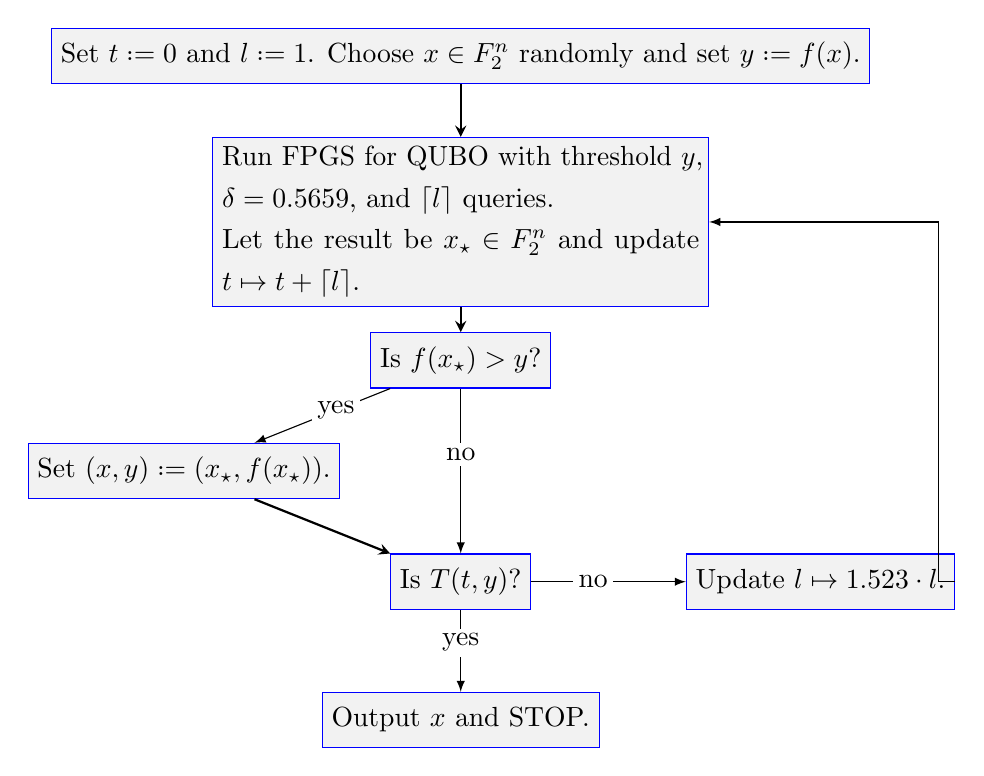
\begin{tikzpicture}[node distance=2em]

   \node[process] (start) {Set $t \eqdef 0$ and $l \eqdef 1$. Choose $x \in \F_2^n$ randomly and set $y \eqdef f \( x \)$.};

   \node[process, below of=start, yshift= -4em] (FPGS) {\parbox{.5\textwidth}{Run FPGS for QUBO with threshold $y$, $\delta = 0.5659$, and $\lceil l \rceil$ queries. \\ Let the result be $x_\star \in \F_2^n$ and update $t \mapsto t + \lceil l \rceil$.}};

   \node[process, below of=FPGS, yshift=-3em] (x_update) {Is $f \( x_\star \) > y$?};

   \node[process, below of=x_update, xshift=-10em, yshift=-2em] (x_update_yes) {Set $\( x, y \) \eqdef \( x_\star, f \( x_\star \) \)$.};

   \node[process, below of=x_update_yes, xshift=10em, yshift=-2em] (fork) {Is $T \( t, y \)$?};

   \node[process, below of=x_update_yes, xshift=23em, yshift=-2em] (l_update) {Update $l \mapsto 1.523 \cdot l$.};

   \node[process, below of=fork, yshift=-3em]  (end) {Output $x$ and STOP.};

   \draw[arrow] (start) -- (FPGS);
   \draw[arrow] (FPGS) -- (x_update);
   \draw[-latex] (x_update) -- node[pos=0.4,fill=white,inner sep=2pt]{yes} (x_update_yes);
   \draw[arrow] (x_update_yes) -- (fork);
   \draw[-latex] (x_update) -- node[pos=0.4,fill=white,inner sep=2pt]{no} (fork);
   \draw[-latex] (fork) -- node[pos=0.4,fill=white,inner sep=2pt]{yes} (end);
   \draw[-latex] (fork) -- node[pos=0.4,fill=white,inner sep=2pt]{no} (l_update);
   \draw[-latex] (l_update) -| ++(1.5, 0) |- (FPGS);

   \end{tikzpicture}}
   \caption{Fixed-point Grover Adaptive Search for QUBO}
   \label{figure:flowchart}
\end{figure}

\bigskip

\begin{comment}
\subsection{Summary of Experiments}

We demonstrate FPGS for IonQ’s Harmony quantum computer with 9 algorithmic all-to-all connected qubits. 6 randomly generated 5-vertice graphs with query complexity of 1 and error bound of $1*10^{-5}$ were tested on Harmony. Several trials for each graph were taken and the trial with highest success probability was recorded for each graph. Because the algorithm is probabilistic and further bounded by some non-zero error, there can be no guarantee of a success probability of \%100. These results were compared with the random probability of measuring cuts above the threshold (ie $N2^{1-v}$) where v represents the number of vertices and N represents the number of cuts above the threshold. The results of these experiments are displayed in FIGURE 1.

\begin{figure}[!h]
   \begin{subfigure}{.5\textwidth}
   \centering
   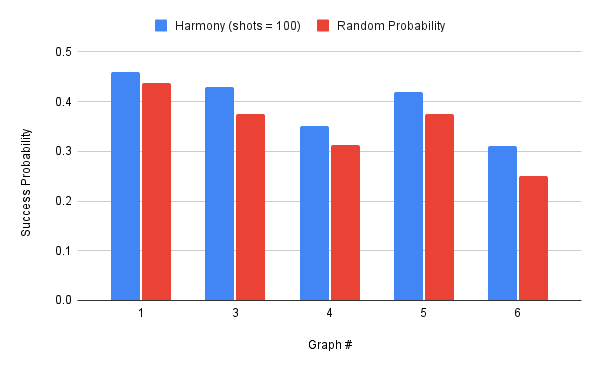
\includegraphics[width=.8\linewidth]{100shotGraph.png}
   \caption{100 shot}
   \label{fig:sfig1}
   \end{subfigure}%
   \begin{subfigure}{.5\textwidth}
   \centering
   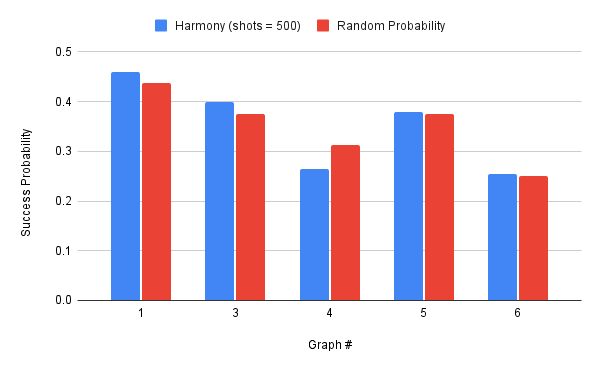
\includegraphics[width=.8\linewidth]{500shotGraph.png}
   \caption{500 shot}
   \label{fig:sfig2}
   \end{subfigure}
   \caption{Success probabilities of Grover's FPS run on IonQ's Harmony with 100 and 500 shots. The measured success probability is shown in blue while the random probability <where eq?> is in red}
   \label{fig:fig}
\end{figure}

At 100 shots, FPGS has a higher probability of finding the maximal cut than by searching randomly. As the shot number increases to 500, this probability decreases and seems to converge with the random probability for graphs 5 and 6. However, neither of these experiments on harmony display significant increased success probability, that is to say, most advantage that the proposed oracle provides is destroyed by the noise present in NISQ devices.

\medskip
\section{Simulation using small graph}
\label{sec:smallgraphs}
   
\end{comment}

\bigskip

\section{Conclusion}
\label{sec:conclusion}

We constructed a marker oracle for QUBO problems with improved complexities to the known previously known designs. These oracles are expected to find uses both Grover-, and QAOA-type methods. We also studied adaptive optimization methods, using our constructions in conjunction with FPGS.
{\color{red} write more}
We conjecture that our Adaptive FPGS for QUBO has a better chance to have provable and (and stronger) performance guarantees, when compared to the original Grover Adaptive Search of \cite{gilliam_grover_2021} (as one only needs to find large enough, but not the exact, $l$) or QAOA (as the number of parameters is lower and their role is more straightforward).

   %========================
   \bibliography{references}
   %========================

\end{document}